\documentclass[a4paper]{article}



    \usepackage[colorinlistoftodos]{todonotes}
 
	\usepackage[utf8]{inputenc}
	\usepackage[T1]{fontenc}
    \usepackage[frenchb]{babel}
    \usepackage{textcomp} 
	\usepackage[top=3cm,left=3cm,right=3cm,bottom=2cm]{geometry}
    \usepackage{lmodern}
    \usepackage{sectsty}
    \usepackage{nicefrac}
	\usepackage{graphicx}
    \usepackage{lastpage}
    \usepackage{fancyhdr}
    \usepackage{amsmath}
    \usepackage{amssymb}
    \usepackage{amsfonts}
    \usepackage{capt-of}
    \usepackage{caption}
    \usepackage{tikz}
    \usepackage{multirow}
    \usepackage{todonotes}
    
    \usepackage{fancyvrb} % pour forcer les verbatim sur une seule page
    \usepackage{url}
    
    \usepackage{subfigure}
    \usepackage{minted}
    \usepackage{multicol}
    \usepackage{array}


    
    \newcommand\matlab{MATLab\textsuperscript{\textregistered}}

\renewcommand{\b}[1]{\boldsymbol{#1}}


\title{Compte rendu de TP: Formation de voies }

\author{Thomas Lechat \& Dinsenmeyer Alice}

\begin{document}
\maketitle



\section{Introduction}

La formation de voies est une méthode d'imagerie acoustique permettant d'obtenir la contribution de sources dans un plan à l'aide d'une antenne de microphones. 

Le principe général est de construire un vecteur de pointage qui pondère les signaux microphoniques en fonction du point d'observation sur le plan source.\\

Ce rapport vise à comparer trois méthodes de formation de voies testées sur des signaux microphoniques obtenus par des mesures de sources connues. 

\section{Obtention des données de test}

Des mesures de champs acoustiques sont effectuées à l'aide d'une antenne constituée de 36 microphones disposés en spirale. Ces microphones sont séparés d'environ $d=10cm$.

Afin d'obtenir un minimum de 2 points de mesures par longueur d'onde $\lambda$, il faut respecter la relation suivante : $$d < \frac{\lambda}{2} ~~~~\Rightarrow~~~~ f < \frac{c}{2d}.$$

L'étude ne peut donc pas être réalisée au-delà de $1715 Hz$.

Les sources sont placées dans un plan situé à 1,43 m de l'axe de l'antenne. La configuration testée est présentée en figure~\ref{exp}.

\begin{figure}[!h]
	\centering
	\caption{Configuration de la mesure : le haut-parleur 1 émet un signal triangle à 600 Hz et l'enceinte 2 émet un bruit blanc.}
		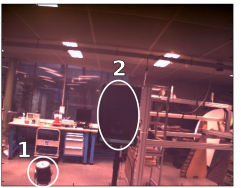
\includegraphics[width=.5\textwidth]{exp.png} 
	\label{exp}
\end{figure}

La matrice interspectrale des microphones appelée $G_{pp}$ peut ainsi être obtenue à l'aide du logiciel Signal Express et du boîtier d'acquisition National Instrument.


\section{Méthodes de formation de voies}

Pour localiser les différentes sources, un programme Matlab (disponible en annexe) est écrit sur la base de trois méthodes de formation de voies. 
\subsection{Méthode de Bartlet}

La méthode de Bartlet consiste à déterminer le vecteur de pointage $\b{w_i}$ tel que l'amplitude estimée des sources $S_i$ s'écrive : $$S_i=\b{w_{i}^{H}p},$$ avec $\b{p}$ les signaux de pression mesurés par les microphones.

Le vecteur $\b{w_i}$ est calculé en minimisant la fonction coût $|\b{w_{i}^{H}p}-A_i|$ où $A_{i}$ sont les amplitudes réelles des sources.

On trouve alors $$\b{w_{i}}=\b{\frac{h_i}{h_{i}^{H}h_{i}}}$$ avec $\b{h_i}$ la contribution de la source i, composée des fonctions de transfert entre chaque microphone m et cette source. Ces fonctions de transfert sont ici celles d'un rayonnement en espace libre sur une distance $r_{mi}$ : $$ h_{mi}=\frac{e^{-jkr_{mi}}}{4\pi r_{mi}}.$$


\subsection{Méthode de Capon}

Dans la méthode de Capon, seule la définition du vecteur de pointage change : on cherche à minimiser $\b{w_{i}^{H}G_{pp}w_{i}}$ avec la contrainte de normalisation $\b{w_{i}^{H}h_i}=1$. 

En résolvant ce problème avec la méthode des multiplicateurs de Lagrange, on trouve le nouveau vecteur de pointage suivant : $$\b{w_i=\frac{G_{pp}^{-1}h_{i}}{h_{i}^{H}G_{pp}^{-1}h_{i}}}.$$\\

Cette méthode est supposée donner de meilleurs résultats que la méthode précédente, mais comporte la contrainte de l'inversion de la matrice $G_{pp}$.

\subsection{Méthode MUSIC}

Cette méthode est basée sur la décomposition en valeurs propres de la matrice interspectrale $G_{pp}$. Cette matrice est ensuite décomposée en un sous-espace signal et un sous-espace bruit. Le sous-espace bruit correspond aux plus petites valeurs propres de $G_{pp}$ et est utilisé pour estimer la présence $P_i$ d'une source au point $i$ :
 \begin{equation}
 P_i = \frac{1}{\sum \limits_{q=r+1}^{M} \frac{\b{\left|h_{i}^{H}u_q\right|^{2}}}{\sigma_{p}^{2}}}
\end{equation}

où $\sigma_q$ sont les valeurs propres de l'espace bruit et $M$ est le nombre de champs cohérents orthogonaux qui composent $G_{pp}$.


\section{Résultats}

Tout d'abord, le contenu global fréquentiel peut être apprécié en observant la moyenne des autospectres de chaque microphone. Sur la figure~\ref{auto}, les deux premiers harmoniques de la source 1 apparaissent clairement à 600 Hz et 1800 Hz, additionnés au bruit blanc de la source 2. \\


Afin d'observer en premier lieu la source de bruit (2), les calculs de localisation sont effectués à 1000 Hz. Ainsi, la source (1) (de fondamental 600 Hz) ne devrait pas être visible.\\

Ensuite, pour localiser la source (1), une étude à 600 Hz est effectuée. Cette source ne peut pas être localisé à l'aide de son deuxième harmonique, car il se situe trop haut en fréquence par rapport à la distance inter-microphonique.\\



\begin{figure}[!h]
	\centering
	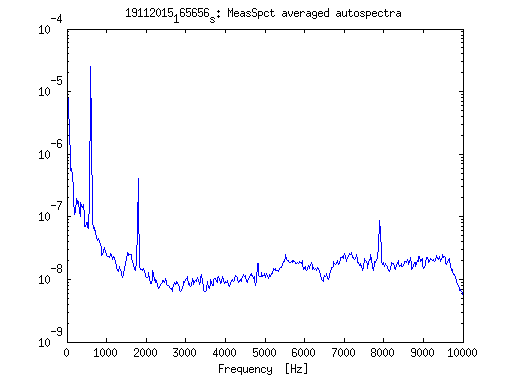
\includegraphics[scale=0.5]{autospectre_16h.png}
	\caption{Moyenne sur chaque microphone de l'autospectre.\label{auto}}
\end{figure}

Les résultats du traitement des données expérimentales sont présentés dans le tableau~\ref{res}.

\begin{table}[!h]
\centering
\hspace{-1cm}
\begin{tabular}{m{.05\textwidth} m{.5\textwidth} m{.5\textwidth} }
 & 600 Hz : Localisation de la source 1  & 1000 Hz : localisation de la source 2 \\
	Capon & 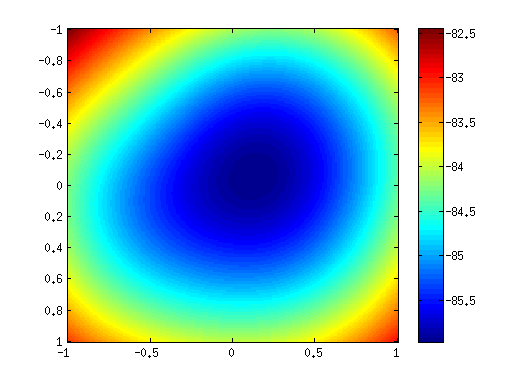
\includegraphics[width=0.5\textwidth]{capon_16h_600hz.png} &\hspace{-2cm} 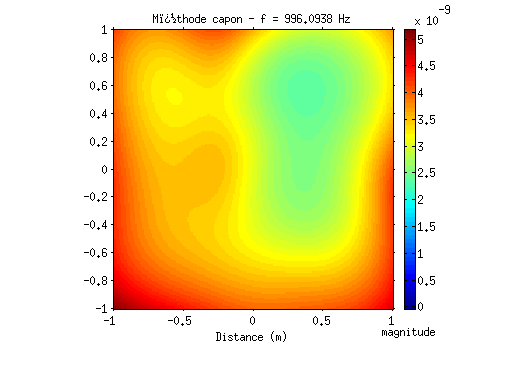
\includegraphics[width=0.5\textwidth]{capon_16h_1000hz.png}\\
	Bartlet & 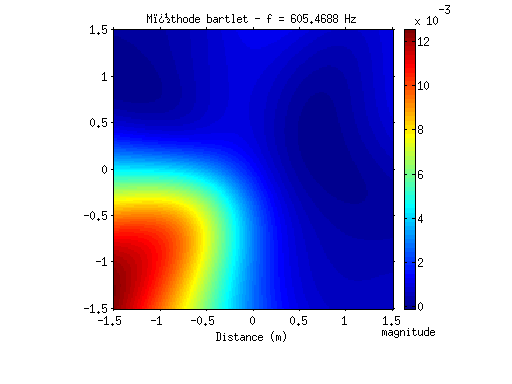
\includegraphics[width=0.5\textwidth]{bartlet_16h_600hz.png} & \hspace{-2cm}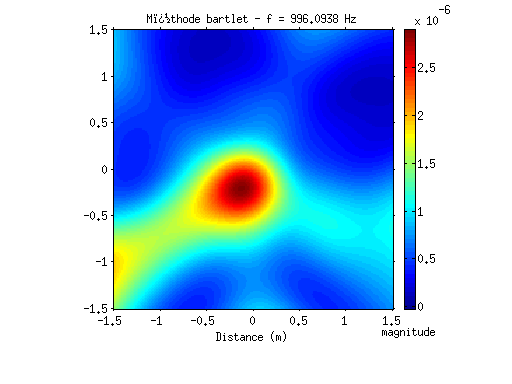
\includegraphics[width=0.5\textwidth]{bartlet_16h_1000hz.png}  \\
	MUSIC & 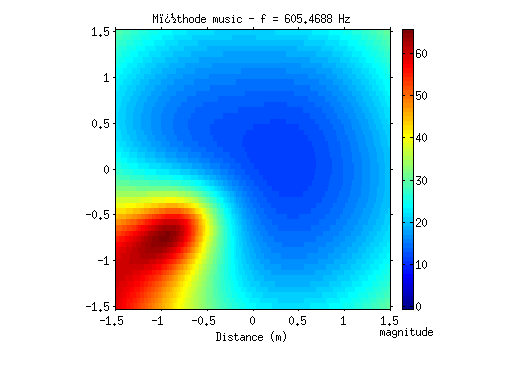
\includegraphics[width=0.5\textwidth]{music_16h_600hz_2.png} &\hspace{-2cm} 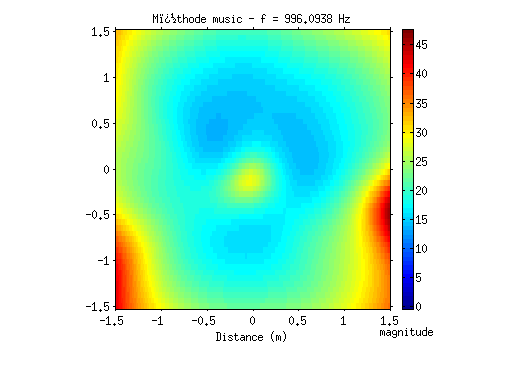
\includegraphics[width=0.5\textwidth]{music_16h_1000hz_5.png} 
\end{tabular}
\caption{Résultats de la localisation de sources pour différentes méthodes à différentes fréquences.\label{res}}
\end{table}


Pour la localisation de la source de bruit (à 1000 Hz), les méthodes de Bartlet et MUSIC permettent de la situer dans le centre du plan source comme attendu. En revanche, la méthode Capon de donne pas de résultats.\\


Les méthodes de Bartlet et MUSIC permettent de localiser grossièrement la source 1 (à 600 Hz). 
Il est difficile de dire si l'absence de la source 2 est due à une résolution spatiale qui ne permet pas de séparer géographiquement les deux sources ou à la différence prononcée de niveau entre les deux sources à 600 Hz (cf figure~\ref{auto}).


 À 600 Hz, la méthode Capon ne donne pas non plus de résultats.\\


De manière générale, la méthode MUSIC semble donner de meilleurs résultats sur la résolution spatiale, mais présente plus d'effets de bords que la méthode Bartlet.\\


\section{Conclusion}

Ce TP a donc permis de découvrir la formation de voie à travers trois méthodes dont les résultats sont mitigés. De meilleurs résultats pourraient être obtenus en approchant les sources de l'antenne ou en augmentant le niveau des sources pour améliorer le rapport signal sur bruit. De plus, en augmentant le temps d'acquisition des mesures, davantage de moyennes auraient pu être effectuées.\\

Peut être est-il possible d'améliorer également les effets de bord par un filtrage adapté.\\





\newpage
\addtolength{\oddsidemargin}{-1cm}
\addtolength{\textheight}{2cm}
\renewcommand{\headsep}{-1cm}
\addtolength{\footskip}{3cm}
\begin{minted}
% bf_traitement
%
% TP Formation de voies
% Jean-Claude Pascal et Jean-Hugh Thomas
%
close all; clear all;
%-- détermination de la méthode : 'bartlet','capon','music'
bfmethod = 'music';

disp(' '), disp(['-- Traitement avec la méthode ',bfmethod]), disp(' ')

%-- construction du path
rootpath = cd;
addpath([rootpath '/Bf_bib']),

%==============================================================================
% Lecture de la matrice interspectrale  (code complet)
%------------------------------------------------------------------------------

%-- Sélection du fichier hdf
%
FilterSpec = {'*.hdf','hdf file'};
[HDFFileName,HDFPathName] = uigetfile(FilterSpec,'load an hdf spectral file');
        
if ischar(HDFFileName)
    filename = [HDFPathName HDFFileName];
else
    return,
end

%-- Visualisation du spectre moyen sur les microphones de l'antenne
%
[avspect,freqvect,axename] = HDFinterface('averageddata',filename);   
HDFinterface('averageddata',filename);

%-- Sélection de la fréquence de traitement
%
disp(' '), disp('Sélection de la fréquence'),
freq = input('     entrer la fréquence à traiter (en Hz) : ');
[freq,ifreq] = nearest(freqvect,freq);

%-- Chargement de la matrice interspectrale
%
[Refarray,axevector,axeorder] = HDFfileAScontrol('getdata',filename,'Refarray',ifreq,':',1);
Gpp = TransRefarray('vec2mat',Refarray,'single');     
Gpp = conj(Gpp);

% INFO : Gpp = Gpp'; dans Matlab Gpp' représente la transposée hermitienne de la matrice complexe Gpp
%        la matrice Gpp est une matrice carrée [M M] (M nombre de microphones)

%==============================================================================
% Lecture des coordonnées des points de l'antenne (code complet)
%------------------------------------------------------------------------------
%
% INFO
% micropnts est une matrice [M 3] où M est le nombre de microphones de l'antenne
% micropnts(:,1) est le vecteur colonne des coordonnées x
% micropnts(:,2) est le vecteur colonne des coordonnées y
% micropnts(:,3) est le vecteur colonne des coordonnées z (normalement nul car le 
% plan de l'antenne est en z = 0)

[micropnts,coordsys,arraysys] = HDFinterface('micropnts',filename);

%==============================================================================
% Détermination du plan de représentation  (code à compléter : donner des valeurs) 
%------------------------------------------------------------------------------

% INFO
% Le plan de représentation est parallèle à celui de l'antenne Pour définir les points 
% où seront estimées les sources il faut fournir les informations suivantes :
%  Nx, Ny -> le nombre de points en x et y
%  dist   -> la distance du plan de représentation à celui de l'antenne
%  Xmin Xmax Ymin Ymax -> les limites du plan de représentation 
% L'origine du repère est située sur l'axe de l'antenne. Par exemple :
Nx = 40;
Ny = 40;
dist = 1.5;
Xmin = -1;
Xmax = 1;
Ymin = -1;
Ymax = 1;
M=size(micropnts);
M=M(1);

%-- construction du maillage sur le plan de représentation
%
x = linspace(Xmin,Xmax,Nx);
y = linspace(Ymin,Ymax,Ny);
[Xmat,Ymat] = meshgrid(x,y);

%-- vecteur [Np 3] des positions des sources
Np = Nx*Ny;
srcpnts = [Xmat(:) Ymat(:) -dist*ones(Np,1)];

%==============================================================================
% Pré-traitement selon la méthode choisie  (code à compléter) 
%------------------------------------------------------------------------------
if strcmpi(bfmethod,'capon')
    disp('   :: pré-traitement pour la méthode de Capon'),
    % INFO
    % le traitement consiste ici à inverser la matrice Gpp
    
    Gpp_inv=Gpp^-1;

elseif strcmpi(bfmethod,'music')
    disp('   :: pré-traitement pour la méthode de MUSIC'),
    % INFO
    % le traitement consiste ici à décomposer la matrice Gpp en utilisant la fonction svd
    % de Matlab [U,S,V] = svd(Gpp)  (dans ce cas particulier V = U')

    [u,s,v] = svd(Gpp);


end    
    
%==============================================================================
% Boucle de traitement pour chacun des points sources  (code à compléter) 
%------------------------------------------------------------------------------
hw = waitbar(0,['traitement méthode ',bfmethod,' ...']);
S = zeros(Np,1);

for ii=1:Np
    
    waitbar(ii/Np,hw);
    
    %-- vecteur [1 3] des coordonnées du point source
    coorsrc = srcpnts(ii,:);
    
    %--------------------------------------------------------------------------
    % Calcul des distances 
    % calcul du vecteur R [M,1] des distance entre chaque microphone et le point 
    % source
    %--------------------------------------------------------------------------
    
    for m=1:M
       R(m)=norm(coorsrc-micropnts(m,:));
    end
    
    
    %--------------------------------------------------------------------------
    % Calcul du vecteur h [M,1] représentant les fonctions de transfert entre 
    % les microphones et le point source (Eqs. 2.2 et 2.3)
    %--------------------------------------------------------------------------
    c=343; %célérité du son dans l'air en m/s
    k=2*pi*freq/c;
    
    h=exp(-j*k*R)./(4*pi*R);
    h=h';
    
    
    %--------------------------------------------------------------------------
    % Calcul du vecteur de pilotage selon la méthode 
    % La méthode MUSIC n'est pas concernée par cette phase
    %--------------------------------------------------------------------------

    if strcmpi(bfmethod,'bartlet')
        % INFO
        % voir Eq. 3.7
    
        w=(h'*h)^(-1)*h;

    elseif strcmpi(bfmethod,'capon')
        % voir Eq. 5.5
    
        w=Gpp_inv*h/(h'*Gpp_inv*h);


    end    
    
    %--------------------------------------------------------------------------
    % Calcul de la distribution des sources selon les méthodes
    % les résultats du calcul sont rangés dans un vecteur S [Np 1]
    %--------------------------------------------------------------------------
    
    if strcmpi(bfmethod,'bartlet')
        % INFO
        % voir Eq. 2.5
    
        S(ii)=w'*Gpp*w; %dsp
        

    elseif strcmpi(bfmethod,'capon')
        % voir Eq. 2.5
    
        S(ii)=w'*Gpp*w; %dsp
        

    elseif strcmpi(bfmethod,'music')
        % voir Eq. 6.3
        somme=0;
        q0=15; %taille de l'espace signal
        for q=q0:M
            somme= somme+ (abs(h'*u(:,q)))^2;
        end
        S(ii)=1/somme; %Pi
         
    end    
    
%------------------------------------------------------------------------------
end % fin de la boucle ii=1:Np

close(hw),
%------------------------------------------------------------------------------


%==============================================================================
% Reconstitution de la matrice rectangulaire et visualisation (code à compléter) 
%------------------------------------------------------------------------------
%
% INFO
% selon meshgrid S doit avoir comme dimensions [Ny Nx]
S = reshape(S,Ny,Nx);
S = real(S);

%-- utiliser ici éventuellement une interpolation pour avoir un maillage de 
%   représentation plus fin  (fonction interp2 de Matlab)
x1 = x;
y1 = y;
S1 = S;

% A COMPLETER EVENTUELLEMENT

%-- visualiser la carte des sources en utilisant la fonction imagesc
%

titre = ['Méthode ',bfmethod,' - f = ',num2str(freq),' Hz'];





reptype = 'lin';  % 'lin' ou 'dB'

if strcmpi(reptype,'lin')
    
%-- pour une représentation linéaire
repstruct.mode = 'mod*';
repstruct.dynscal = [];   %  -> range of representation of scalar map (used for dB)
repstruct.maxscal = [];    %  -> max value of scalar map ( [] -> automatic scaling)
repstruct.stepscal = 10;   %  -> step for rounded max value in automatic scaling
repstruct.dBref = 1;       %  -> energy reference for dB (A = 10 log [real(Z)/dBref])
repstruct.title = titre;   %  -> map title string
repstruct.underrangecolor = [0.9 0.9 0.9]; %  -> underrange color
repstruct.unit = '';       %  -> string of quantity unit to put under the colorbar

else
    
%-- pour une représentation en dB
Dyn = 15;
RefdB = 1e-12;
repstruct.mode = 'dB*';
repstruct.dynscal = Dyn;   %  -> range of representation of scalar map (used for dB)
%repstruct.maxscal = dBmax; %  -> max value of scalar map ( [] -> automatic scaling)
repstruct.maxscal = [];   %  -> max value of scalar map ( [] -> automatic scaling)
repstruct.stepscal = 1;    %  -> step for rounded max value in automatic scaling
repstruct.dBref = RefdB;   %  -> energy reference for dB (A = 10 log [real(Z)/dBref])
repstruct.title = titre;   %  -> map title string
repstruct.underrangecolor = [0.95 0.95 0.95]; %  -> underrange color
repstruct.unit = 'dB';     %  -> string of quantity unit to put under the colorbar

end

figure
%imagesc(x1,y1,S1)
ccmap(repstruct,x1,y1,S1);



\end{minted}


\end{document}